\documentclass[xcolor=x11names,compress,professionalfonts]{beamer}

%% General packages %%%%%%%%%%%%%%%%%%%%%%%%%%%%%%%%%%
\usepackage[utf8]{inputenc}
\usepackage{psfrag}
\usepackage{graphicx}
\usepackage{tikz}
\tikzset{% change default arrow tips
    >=latex
}
\usepackage{ifthen}

\usepackage{amsmath}
\usepackage{nicefrac}

\usepackage{color}

%%%%%%%%%%%%%%%%%%%%%%%%%%%%%%%%%%%%%%%%%%%%%%%%%%%%%%


%% Beamer Layout %%%%%%%%%%%%%%%%%%%%%%%%%%%%%%%%%%
\useoutertheme[subsection=false,shadow]{miniframes}
\useinnertheme{rectangles}

\setbeamertemplate{navigation symbols}{}%remove navigation symbols

\newcommand{\btVFill}{\vskip0pt plus 1filll}%place an element at the bottom of the page

\usepackage{libertine}
\usepackage[T1]{fontenc}

\setbeamerfont{title like}{shape=\scshape}
\setbeamerfont{frametitle}{shape=\scshape}

\setbeamercolor*{lower separation line head}{bg=DeepSkyBlue4} 
\setbeamercolor*{normal text}{fg=black,bg=white} 
\setbeamercolor*{alerted text}{fg=red} 
\setbeamercolor*{example text}{fg=black} 
\setbeamercolor*{structure}{fg=black} 
 
\setbeamercolor*{palette tertiary}{fg=black,bg=black!10} 
\setbeamercolor*{palette quaternary}{fg=black,bg=black!10} 

\renewcommand{\(}{\begin{columns}}
\renewcommand{\)}{\end{columns}}
\newcommand{\<}[1]{\begin{column}{#1}}
\renewcommand{\>}{\end{column}}

\definecolor{BostonBlue}{HTML}{00688B}
\definecolor{Complementary}{HTML}{8B2300}

\renewcommand{\ss}[1]{\scriptsize{\text{#1}}}
%%%%%%%%%%%%%%%%%%%%%%%%%%%%%%%%%%%%%%%%%%%%%%%%%%

\usepackage{braket}
% compile child documents using this preamble
\usepackage{subfiles}

%%%My Math

\newcommand{\pd}[2]{\frac{\displaystyle \partial #1}{\displaystyle\partial #2}} % for partial derivatives
\renewcommand{\d}[1]{\mathrm{d}#1}

\begin{document}

\begin{frame}
\title{États électroniques fractals sur des quasicristaux}

\author{ Nicolas Macé, Anuradha Jagannathan, \\ Frédéric Piéchon, Rémy Mosseri}

\institute % (optional)
{
  Laboratoire de Physique des Solides, Université Paris-Sud \\
  Laboratoire de Physique Théorique de la Matière Condensée, UPMC
}

\date{21 Février 2017}

\titlepage

\btVFill
\centering
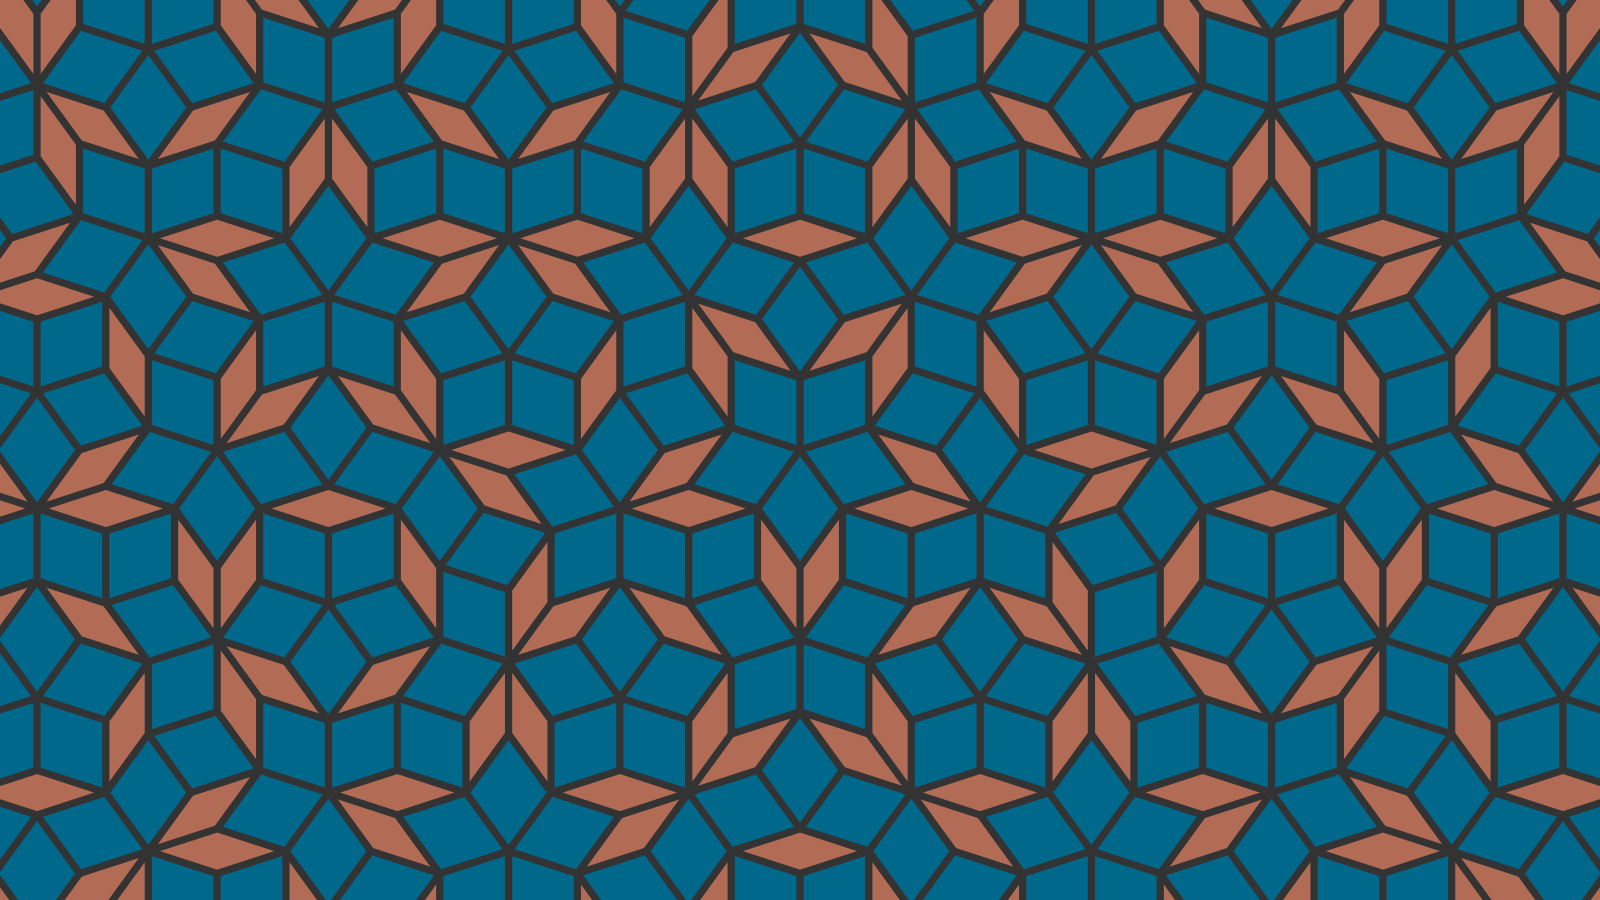
\includegraphics[scale=0.09]{img/cover.png}

\end{frame}

\begin{frame}
\frametitle{Outline}
\tableofcontents[hideallsubsections]
\end{frame}

\section{La structure des quasicristaux}
%Each section needs a subsection for the small points on top to show up
\subsection{Dummy}
\begin{frame}{Les quasicristaux ?}
Un arrangement apériodique mais ``ordonné'' d'atomes/molécules/colloïdes

Plus précisément, un quasi a les propriétés suivantes :
\begin{itemize}
	\item il est \textbf{apériodique}
	\item il présente \textbf{un ordre à longue distance} (la figure de diffraction possède des pics nets).
\end{itemize}
Notion de récurrence $\to$ les \textbf{pavages quasipériodiques} modélisent les quasis.
(voir \textit{Baake \& Grimm, Aperiodic Order (2013)})
\(
	\<{6cm}
		\centering
		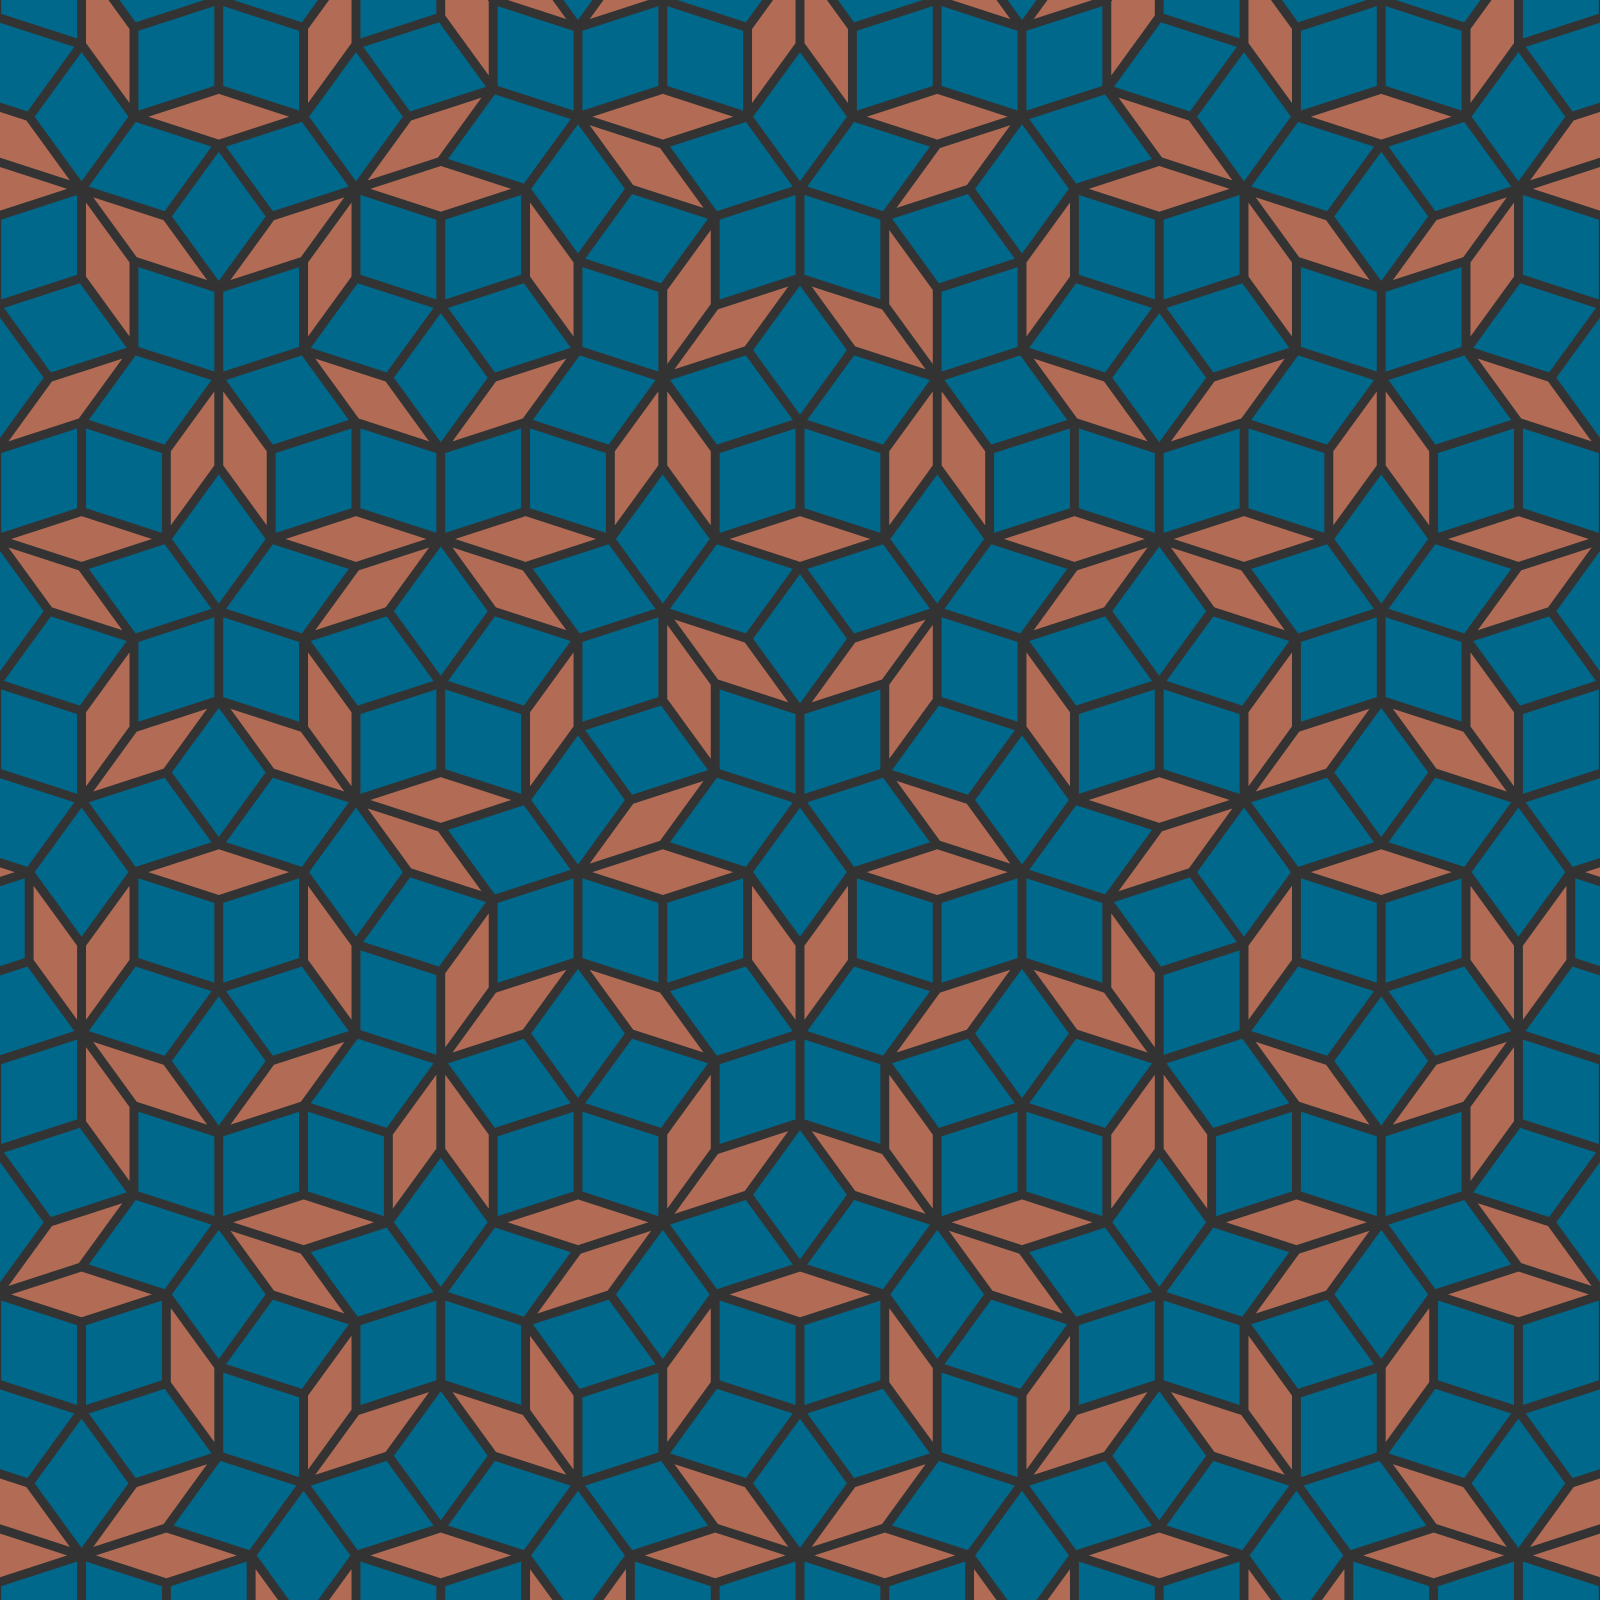
\includegraphics[scale=0.06]{img/penrose.png}
		
		\ss{Un morceau du pavage de Penrose,} \ss{souvent utilisé pour modéliser les quasis.}
	\>
	\<{6cm}
		\centering
		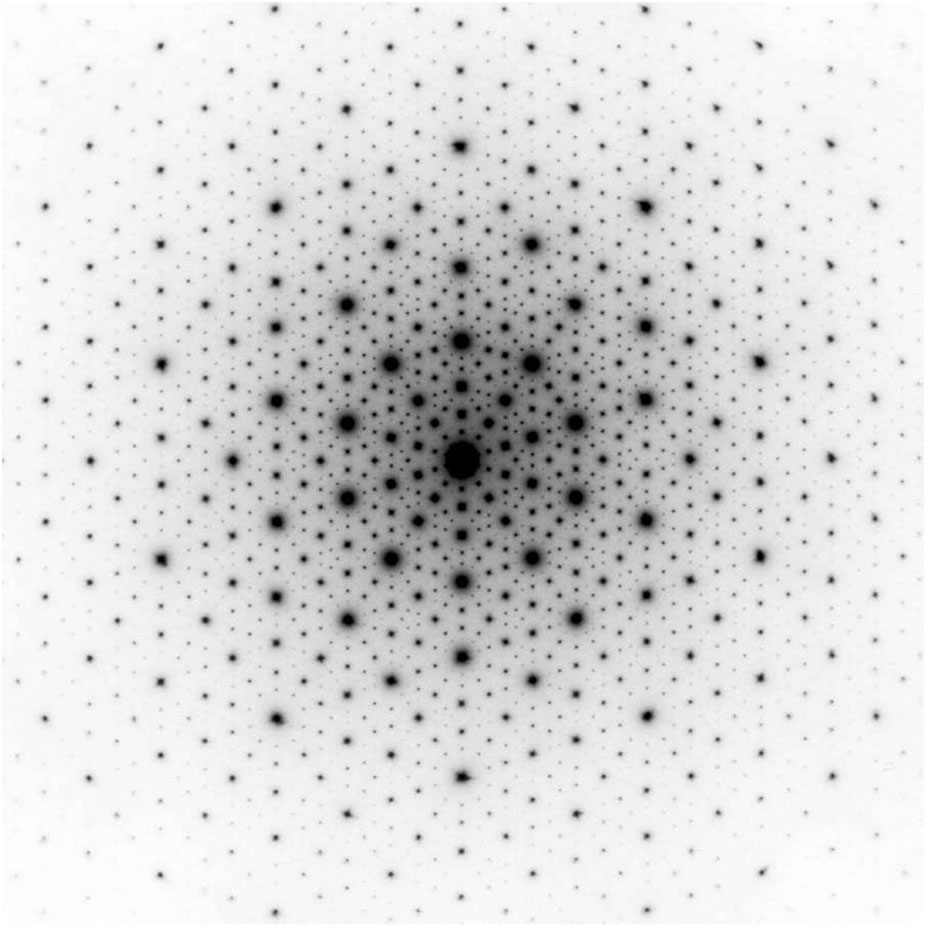
\includegraphics[scale=0.1]{img/diffraction_tenfold.png}
		
		\ss{Figure de diffraction d'un alliage d'AlPdMn} \ss{(groupe de Conradin Beeli)}
	\>
\)
\end{frame}

\begin{frame}{Exemples de quasicristaux}
\(
	\<{6cm}
		\centering
		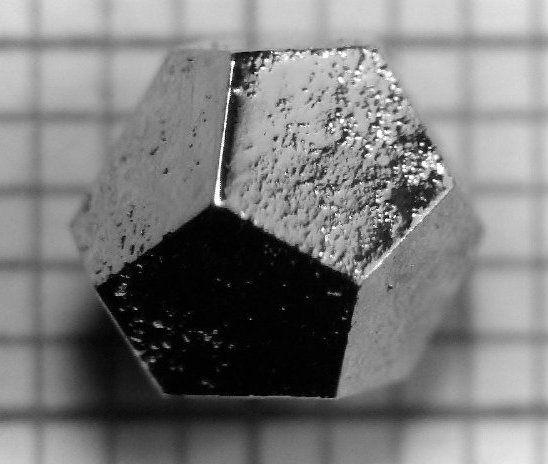
\includegraphics[scale=0.28]{img/homgzn.png}
		
		\ss{L'alliage HoMgZn alloy dans sa phase icosahédrale} \ss{(voir \url{doi:10.1038/nmat1244})}
	\>
	\<{6cm}
		\centering
		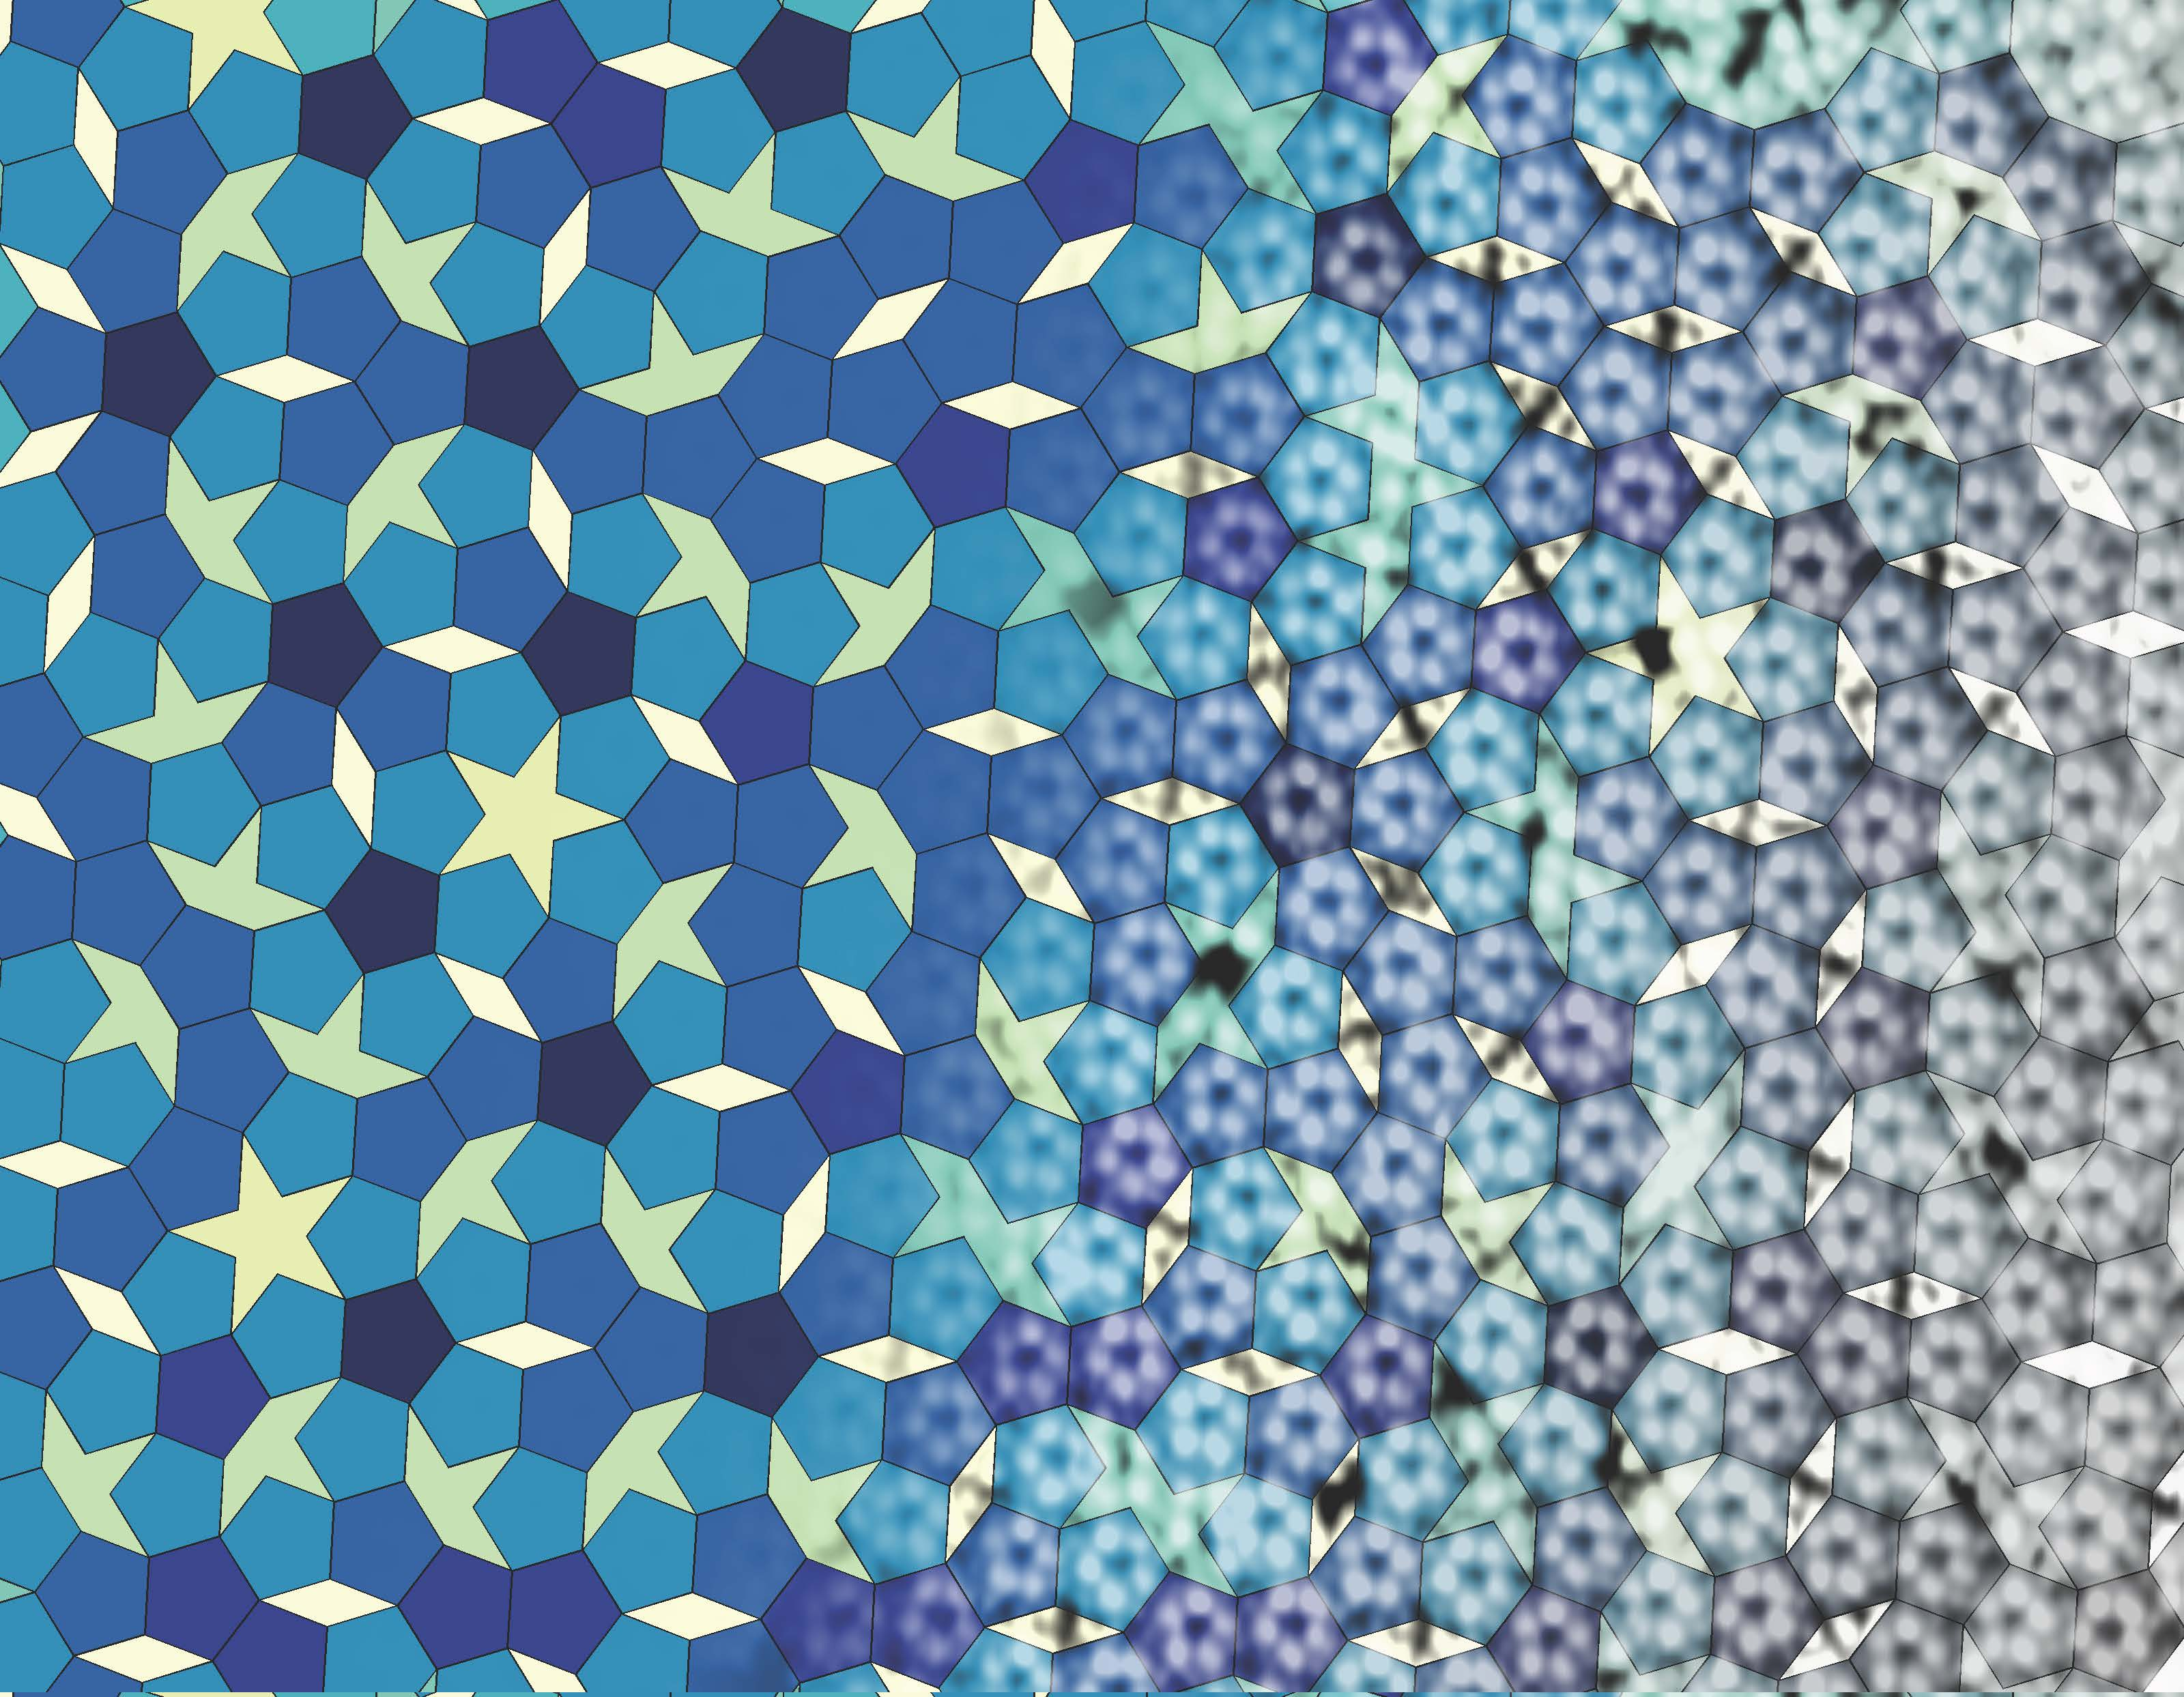
\includegraphics[scale=0.22]{img/wasio.jpg}
		
		\ss{Un quasicristal 2D de molécules} \ss{(voir \url{doi:10.1038/nature12993})}
	\>
\)

\begin{itemize}
	\item De nombreux alliages métalliques sont quasicristallins sous de bonnes conditions
	\item Seul exemple connu dans la nature: la météorite de Khatyrka  (voir \url{doi:10.1126/science.1170827 }). 
\end{itemize}
\end{frame}

\section{Un électron sur une chaîne}
%Each section needs a subsection for the small points on top to show up
\subsection{Dummy}
\begin{frame}{Conduction électrique d'une chaîne d'atomes}


\(
	\<{6cm}
		\centering
		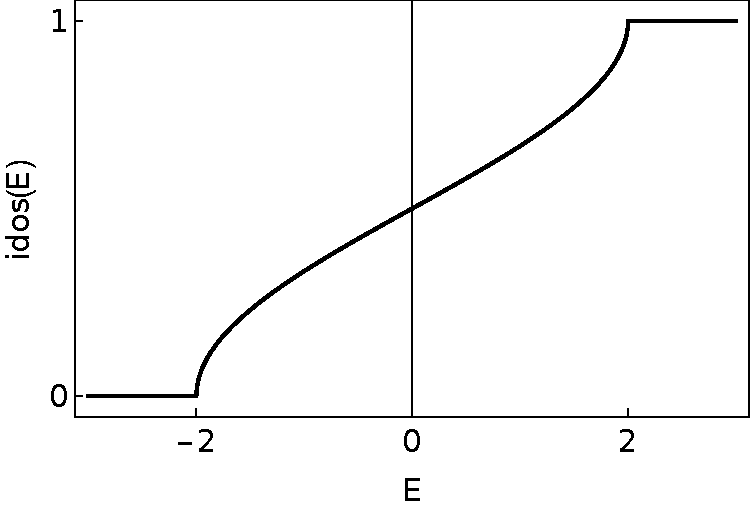
\includegraphics[scale=0.4]{img/idos_chaine_periodique.pdf}
		
		\ss{Densité d'états intégrée de la chaîne périodique}
		\ss{(Amplitude de saut $t=1$)}
	\>
	\<{6cm}
		\centering
		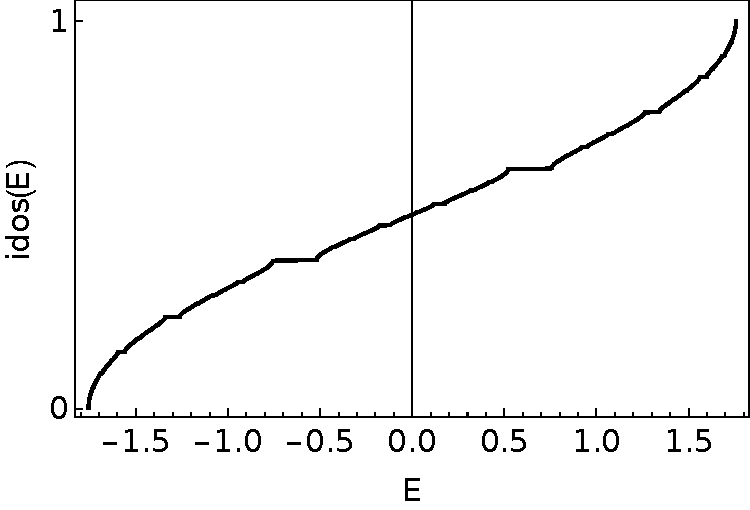
\includegraphics[scale=0.4]{img/idos_fibo.pdf}
		
		\ss{Densité d'états intégrée de la chaîne de Fibonacci} 
		\ss{(Amplitudes de saut $t_B = 1$, $t_A = 0.8$)}
		%\ss{(see \url{doi:10.1007/BF01127714})}
	\>
\)

\(
	\<{6cm}
		\centering
		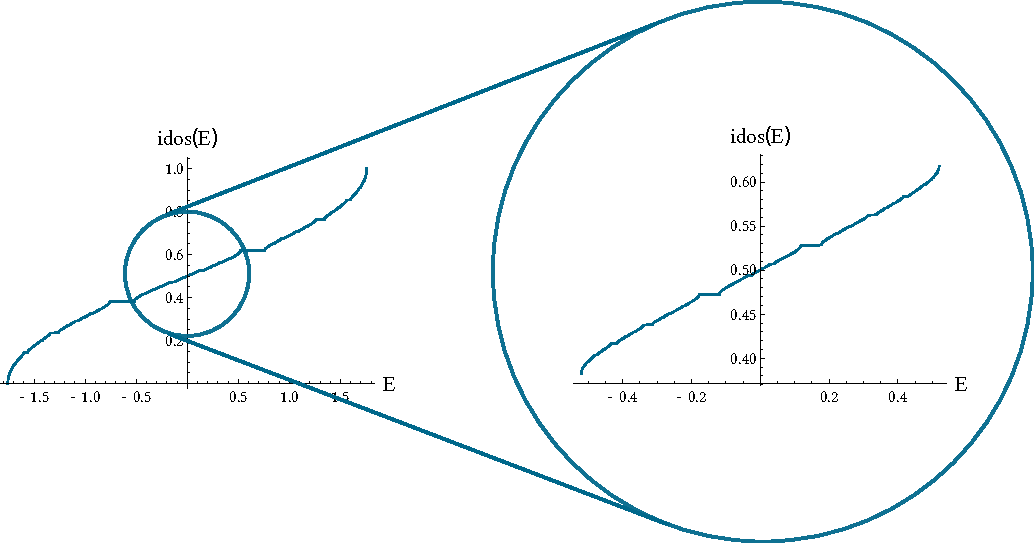
\includegraphics[scale=0.35]{img/idos.pdf}
	\>
	\<{6cm}
\begin{itemize}
	\item Le courant passe si $E_\text{incident} \notin \text{plateau de l'idos}$.
	\item Chaîne périodique : courant si $E_\text{incident} \in [-2t, 2t]$.
	\item Chaîne quasi : courant si $E_\text{incident} \in \text{ensemble de Cantor}$ (voir \emph{Niu \& Nori, PRB 1990})
\end{itemize}
	\>
\)

\end{frame}

\begin{frame}{État central d'une chaîne}

{\centering
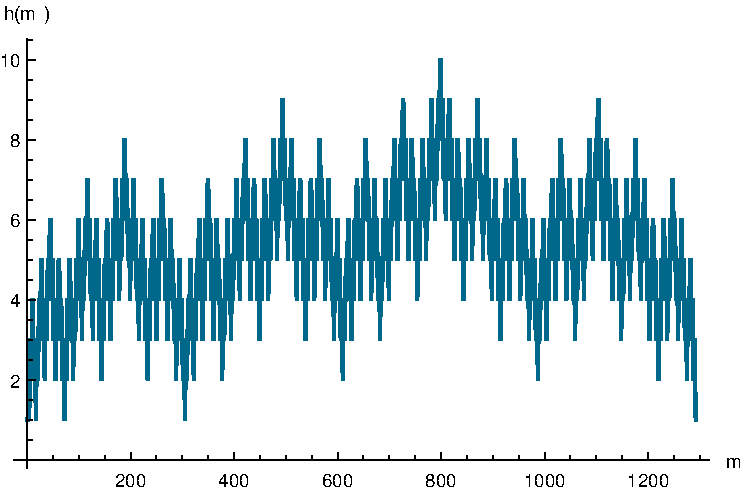
\includegraphics[scale=.7]{img/heights.pdf}

\ss{La fonction de hauteur sur un morceau de la chaîne de Fibonacci}

}

\begin{itemize}
	\item La fonction flèche est quasipériodique.
	\item Son intégrale, la fonction de hauteur, croît en $\sqrt{\log m}$.
\end{itemize}
\end{frame}

\begin{frame}{État central}

{\centering
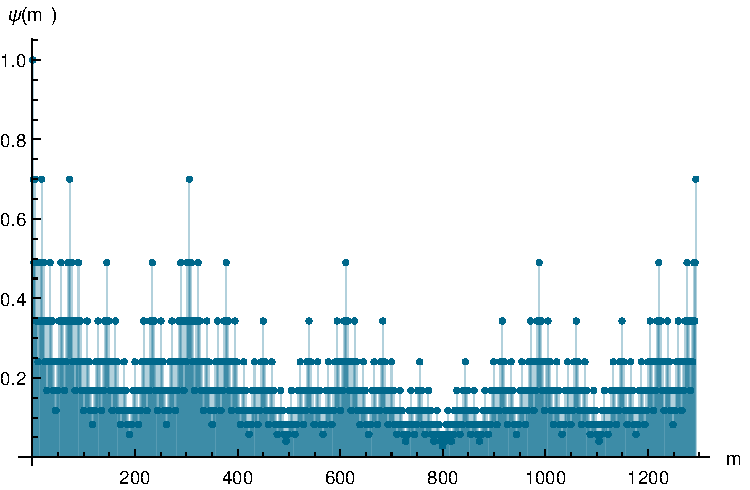
\includegraphics[scale=.8]{img/wavefunction.pdf}

}

\end{frame}

\begin{frame}{Dimensions fractales}

(voir \emph{Halsey et al., Fractal measures and their singularities (1986)})

{\centering
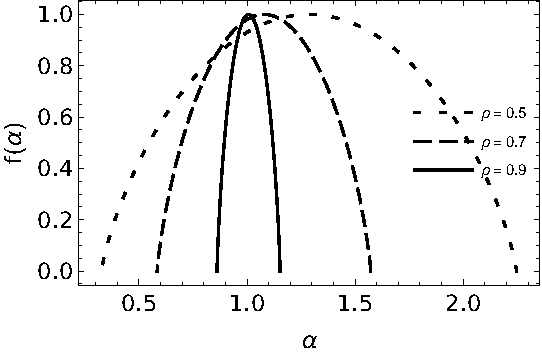
\includegraphics[scale=1.]{img/multifractal_spectrum_fibo.pdf}

}
\begin{itemize}
	\item État central critique (ni localisé ni étendu).
	\item ``de moins en moins'' critique à mesure que $\rho \to 1$.
\end{itemize}
\end{frame}

\begin{frame}{Coefficient de transmission}

$T(L)$ : fraction du courant traversant un morceau $L$ de chaîne.

(voir \emph{Beenakker, Random-matrix theory of quantum transport (1997)})

{\centering
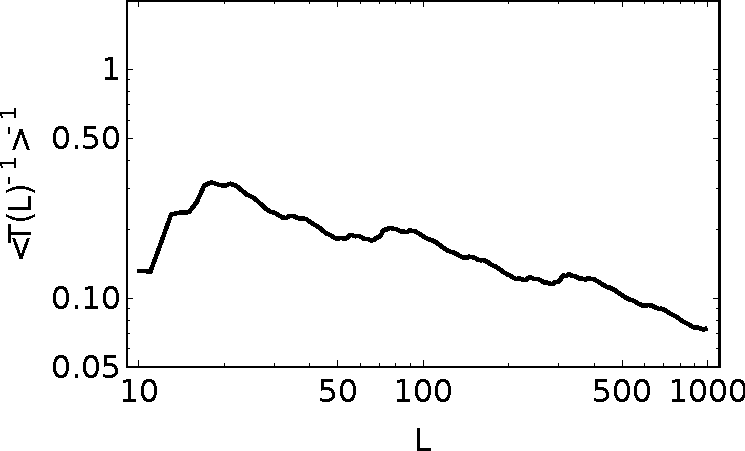
\includegraphics[scale=.8]{img/harmonic_mean_transmission.pdf}

}
$\to$ la transmission décroît lentement avec la taille (loi de puissance).
\end{frame}

\begin{frame}{Récap et questions ouvertes}

Récap
\begin{itemize}
	\item État central : \textbf{fonction flèche} quasipériodique,
	\item croissance lente de son intégrale, la \textbf{fonction de hauteur},
	\item $\to$ état central \textbf{critique}.
	\item Fonction de hauteur simple $\to$ accès à des quantités physique (ex. \textbf{transmission}).
\end{itemize}
$\rightarrow$ Ces conclusions restent valides pour les modèles 2D.

Questions ouvertes
\begin{itemize}
	\item Autres états ? (chaîne périodique perturbée $\to$ période effective $\to$ fonction flèche)
	\item Qu'est-ce qu'une fonction flèche ? (substitution ? coupe et projection ?)
	\item Dans quel espace vivent les états électroniques ?
\end{itemize}
\end{frame}

\begin{frame}{Coupe et projection : construction par Klötze}

	\centering
	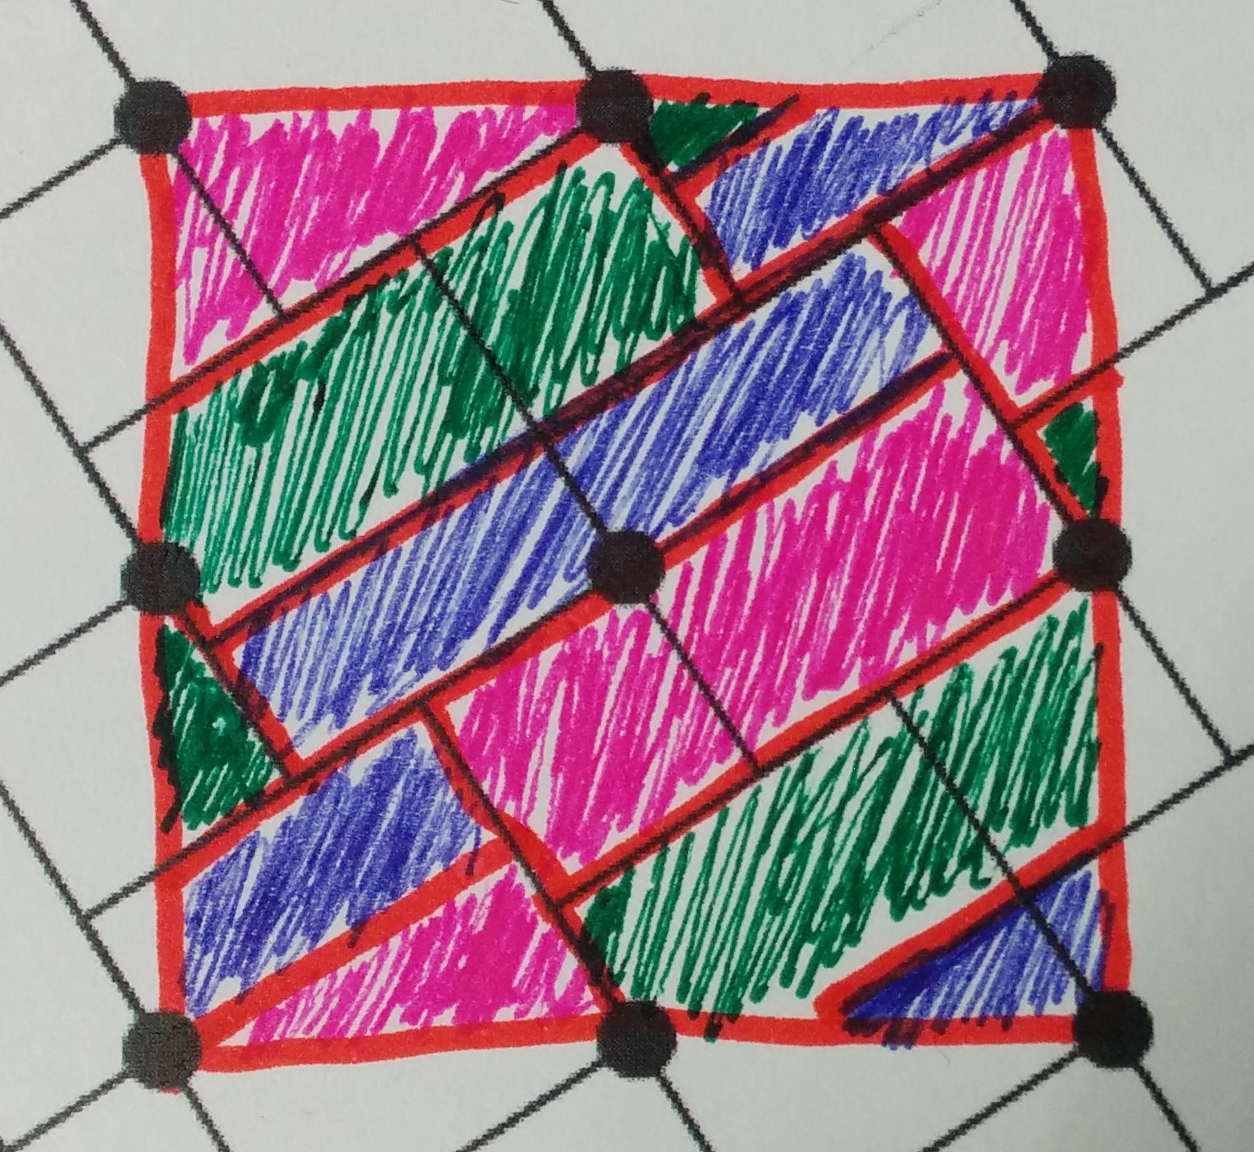
\includegraphics[scale=0.1]{img/klotz_heights.png}
	~~~~~~~~~~~~~
	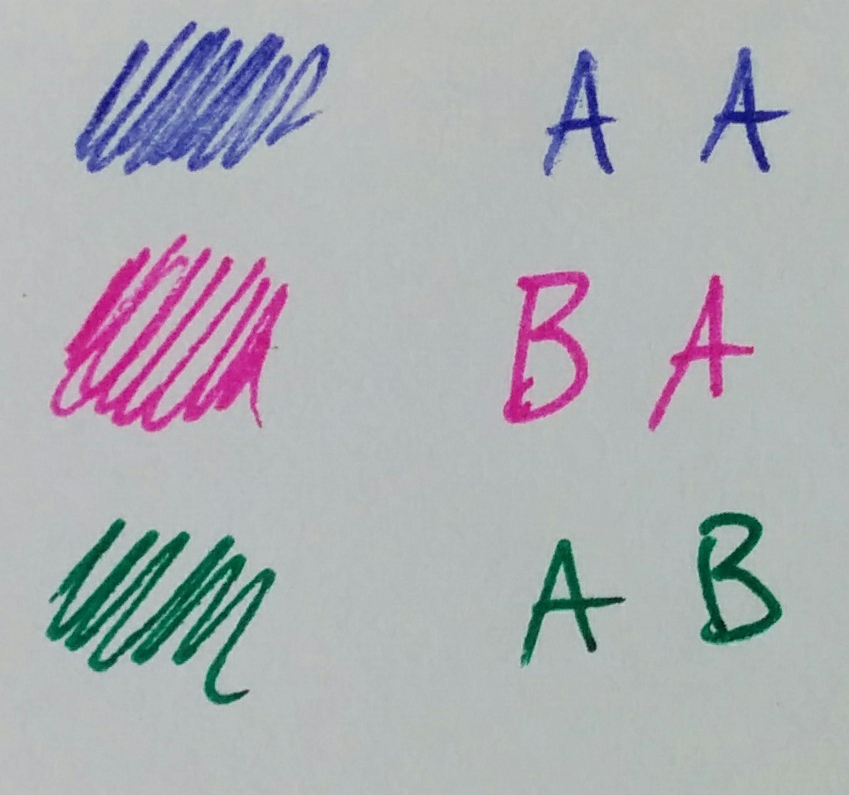
\includegraphics[scale=0.1]{img/klotz_heights_legend.png}	

Les Klötze du champ de flèches de l'état central.

\flushleft{(voir \emph{Kramer \& Schlottmann, J. Phys. A: Math. Gen. (1989)})}
\end{frame}

\begin{frame}{Un résultat négatif sur l'état en bord de spectre}

{\centering
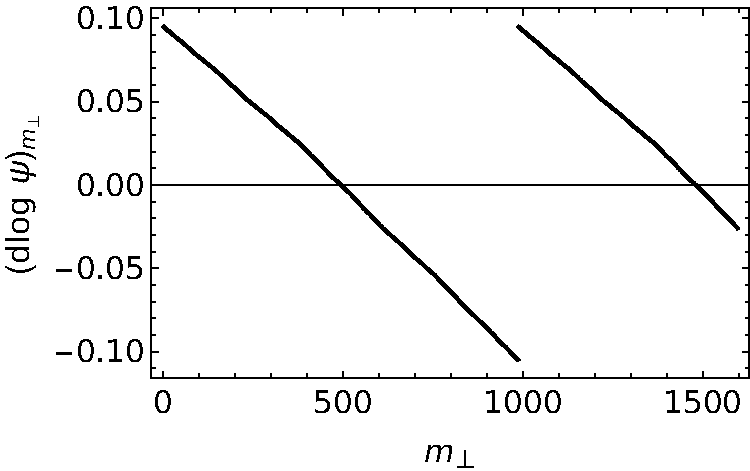
\includegraphics[scale=.8]{img/state_spec_edge.pdf}

}
$\to$ pas de champ de flèches local.

\end{frame}

\section{Un électron sur un pavage quasipériodique}
\subsection{Dummy}
\begin{frame}{Deux pavages quasipériodiques}
\(
	\<{6cm}
		\centering
		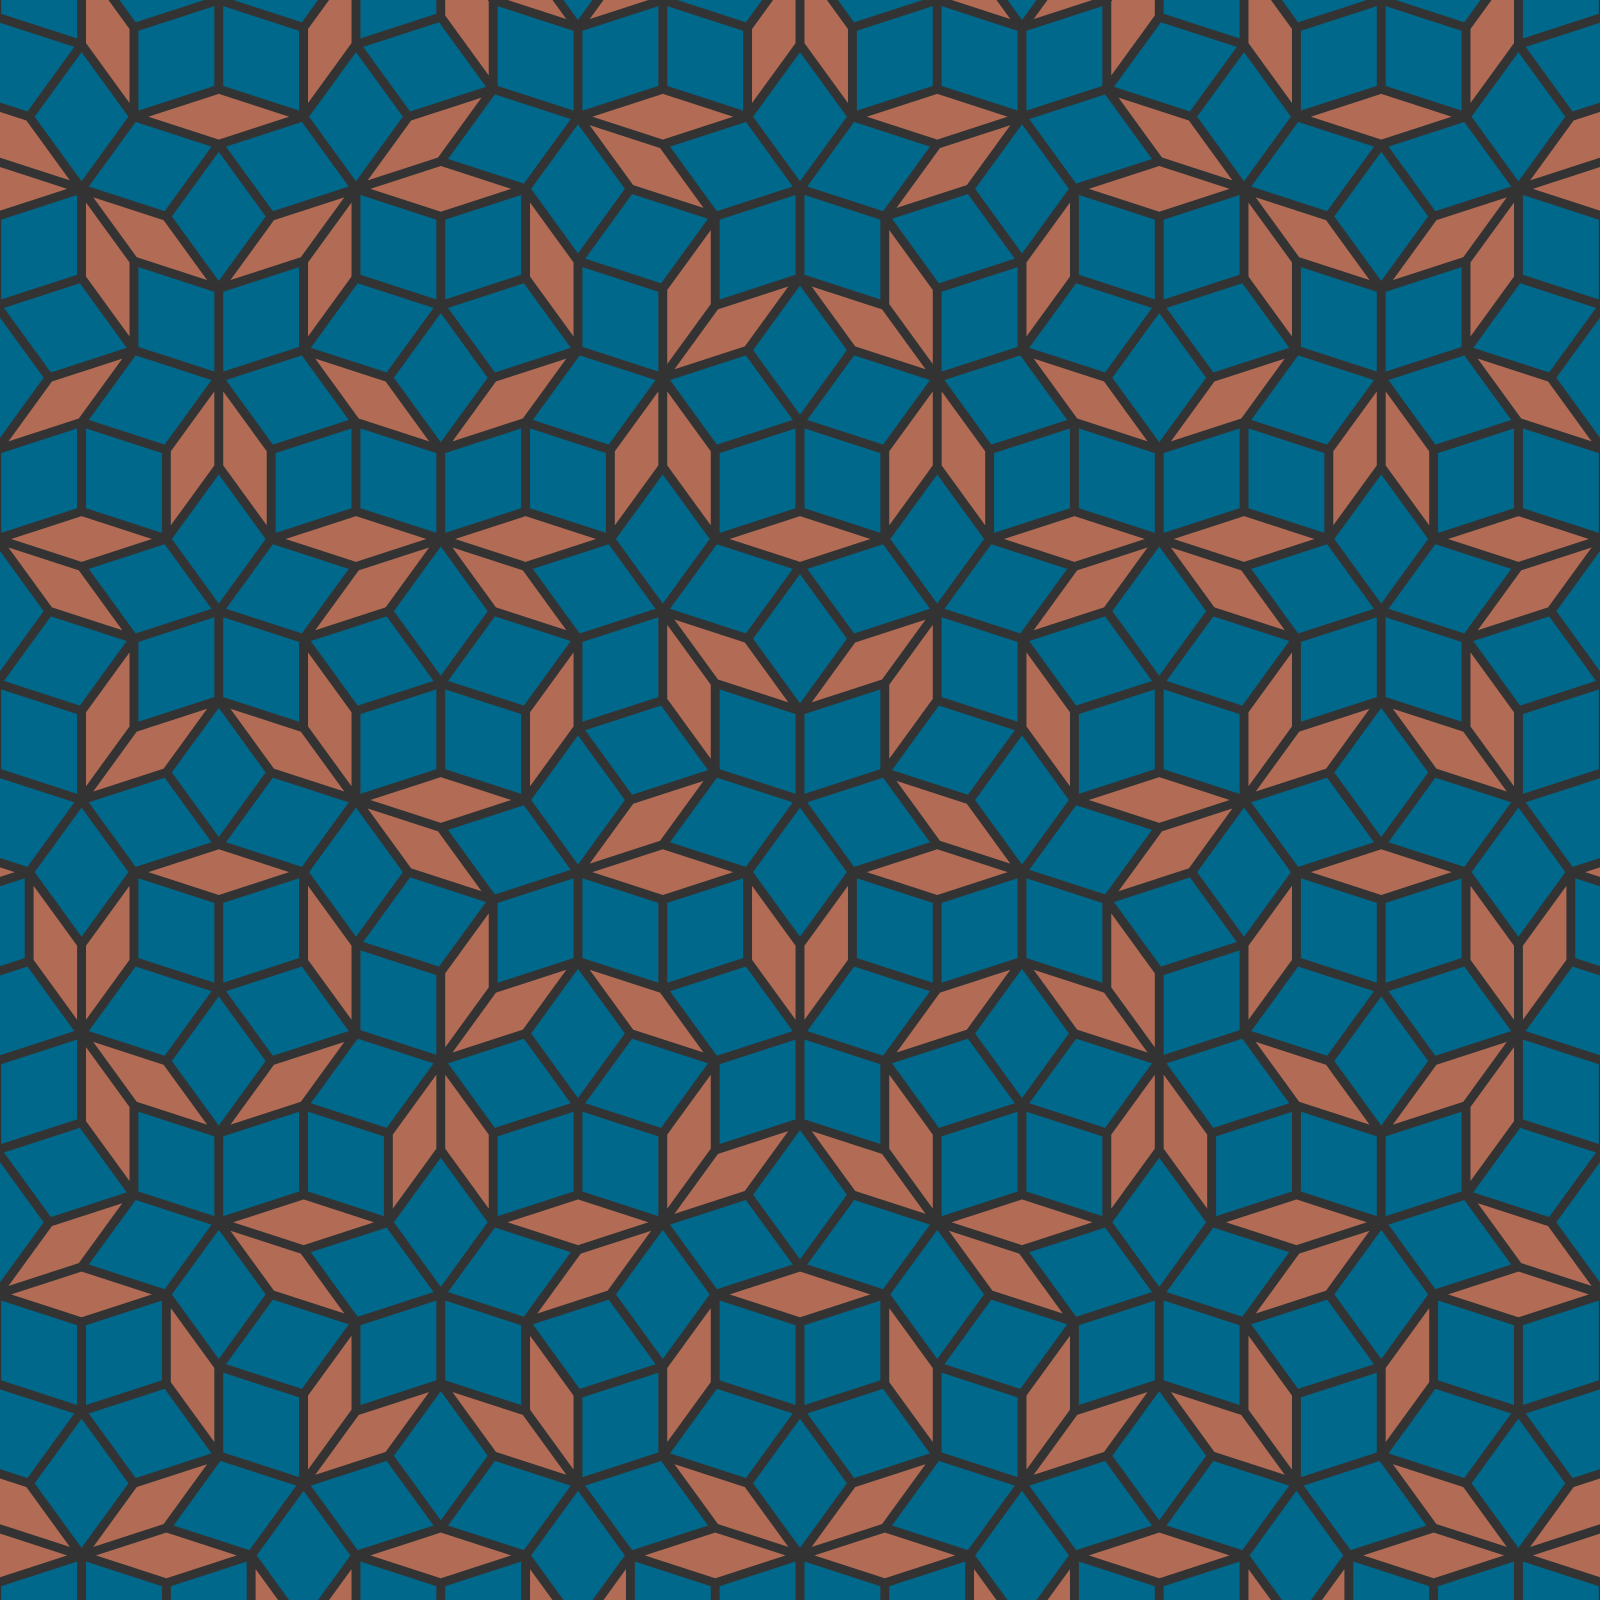
\includegraphics[scale=0.06]{img/penrose.png}
		
		\ss{Pavage de Penrose}
		
		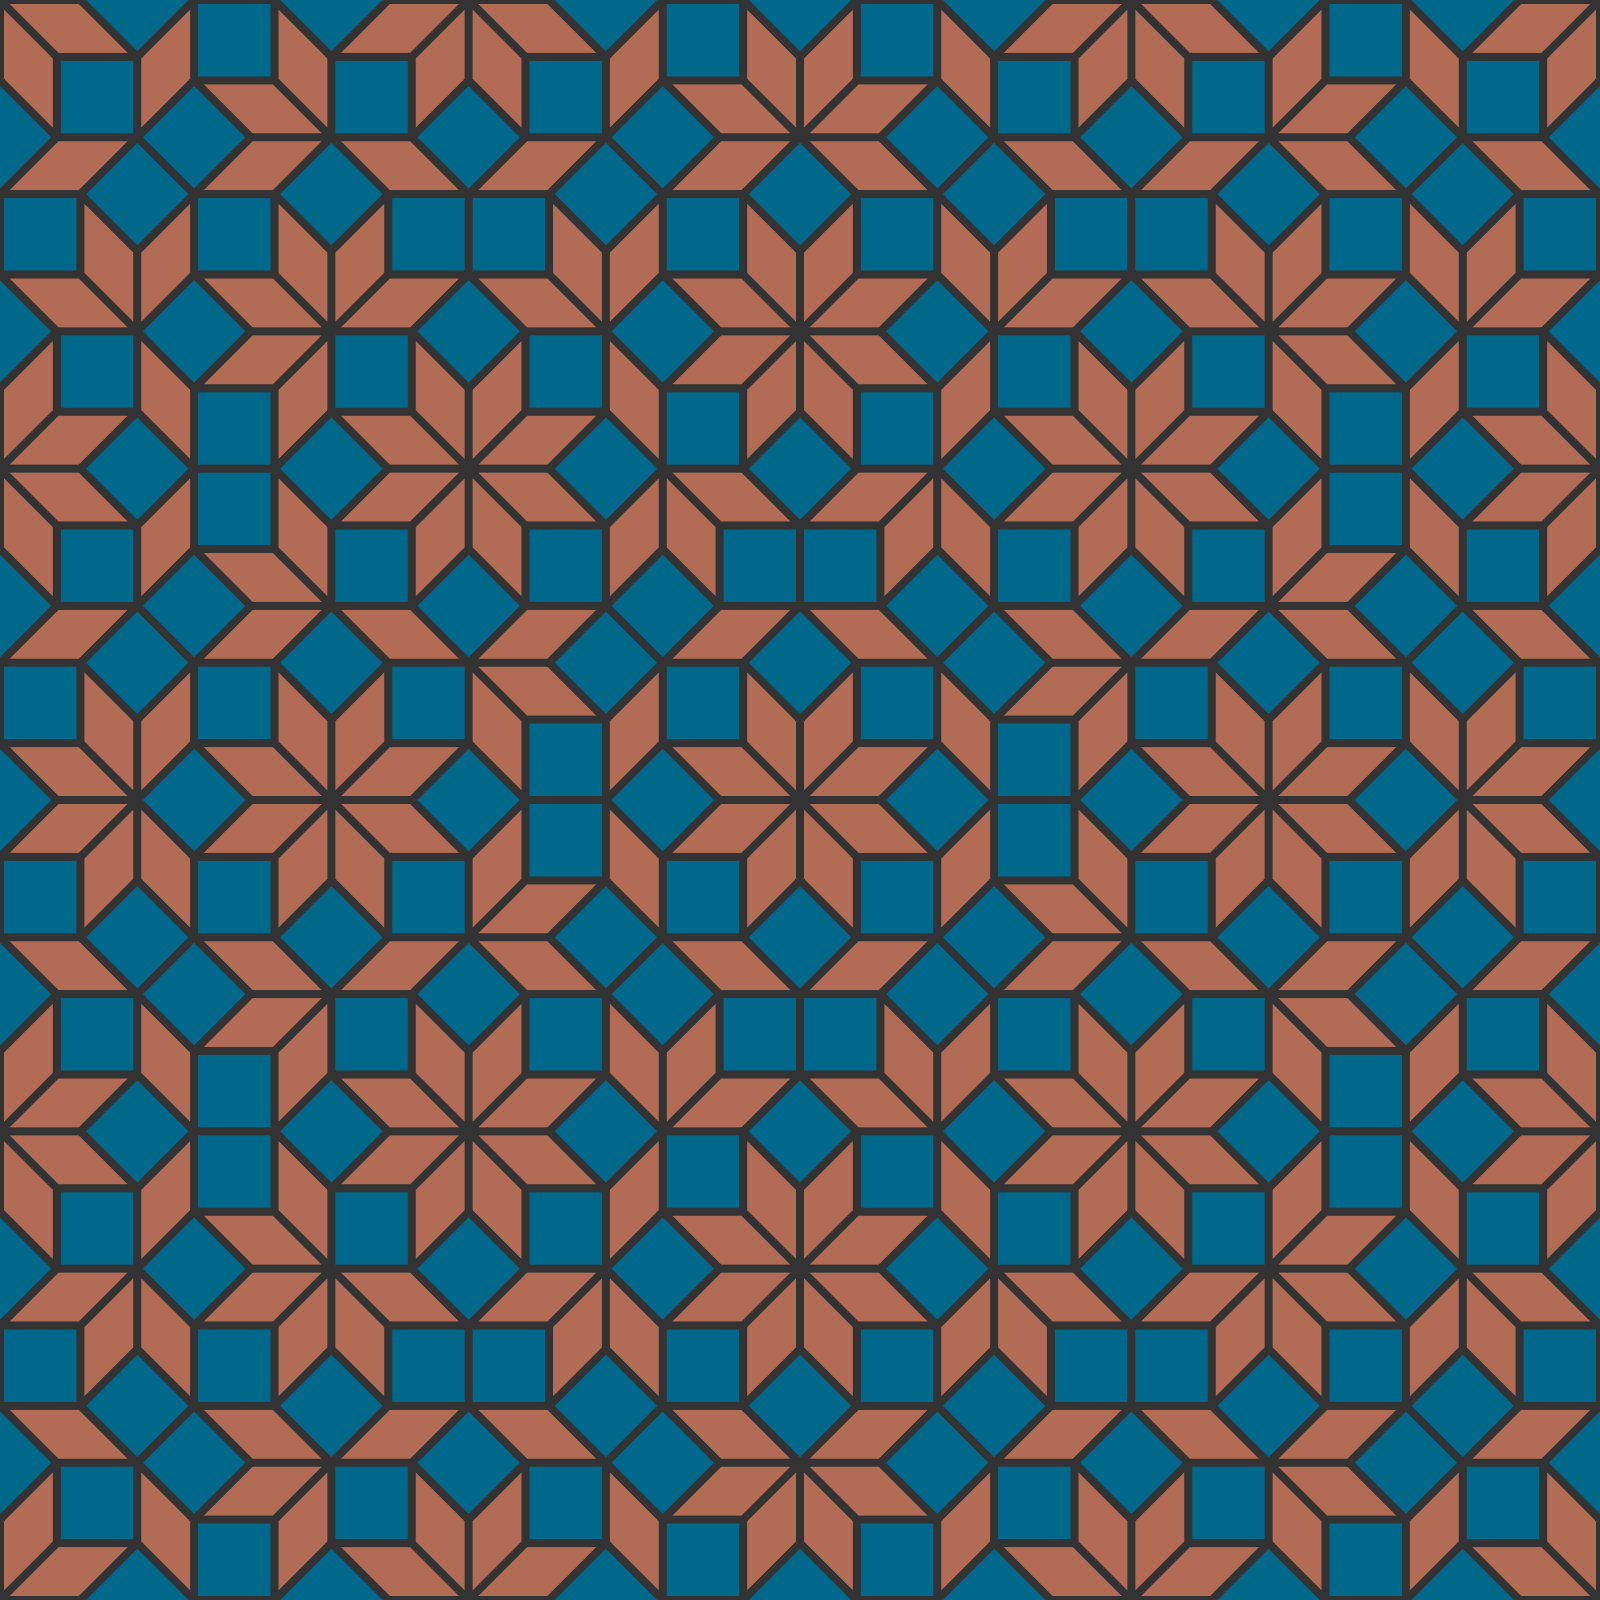
\includegraphics[scale=0.06]{img/ammann-beenker.png}
		
		\ss{Pavage d'Ammann-Beenker}
	\>
	\<{6cm}
		\centering
		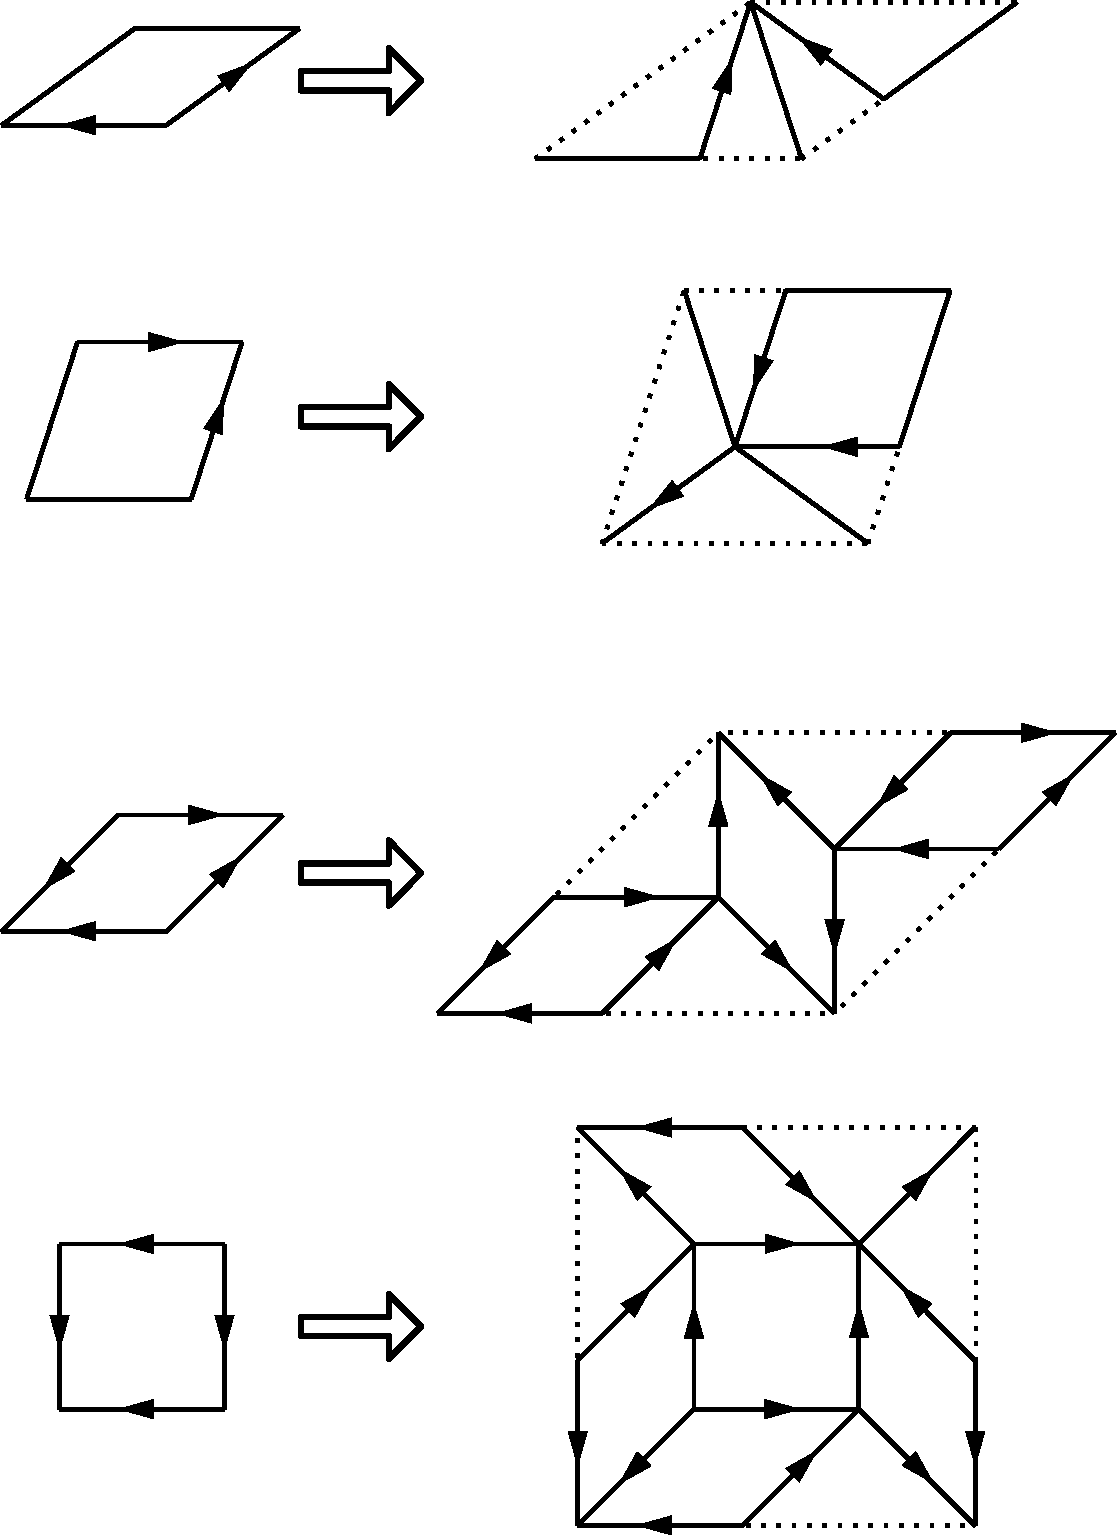
\includegraphics[scale=0.25]{img/inflation_rules}
		
	\>
\)
\end{frame}

\begin{frame}{Méthode de coupe et projection}
\centering
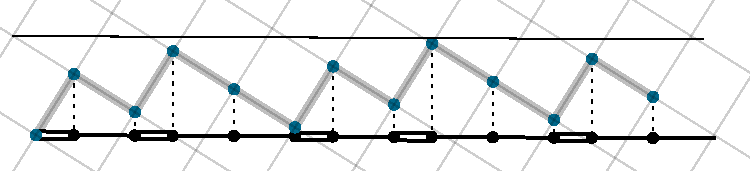
\includegraphics[scale=.8]{img/cut_and_project_Fibonacci.pdf}
\end{frame}

\end{document}